Word2vec --- общее название для совокупности моделей на основе искусственных нейронных сетей, предназначенных для получения
векторных представлений слов на естественном языке. Используется для анализа семантики естественных языков, основанный
на дистрибутивной семантике, машинном обучении и векторном представлении слов. Программное обеспечение под названием
<<Word2vec>> было разработано группой исследователей Google в 2013 году \cite{mikolov-etal-2013-linguistic,mikolov2013efficient}.
Подобные модели и инструменты разрабатывались и ранее, еще в 2000-х годах (\cite{bengio2003neural,collobert2008}),
однако первой популярной реализацией векторно-семантической модели стала именно Word2vec.

Заметим, что ошибочно называть Word2vec алгоритмом --- в совокупности реализованы два основных алгоритма обучения:
CBoW (англ. Continuous Bag of Words, <<непрерывный мешок со словами>>, англ. bag --- мультимножество)
и Skip-gram.

CBoW --- архитектура, которая предсказывает текущее слово, исходя из окружающего его контекста. С другой стороны, архитектура
типа Skip-gram действует наоборот: она использует текущее слово, чтобы предугадывать окружающие его слова.
Построение модели word2vec возможно с помощью двух данных алгоритмов.
Порядок слов контекста не оказывает влияния на результат ни в одном из этих алгоритмов.

Архитектура модели CBoW пытается предсказать текущее целевое слово (центральное слово) на основе исходных контекстных слов
(окружающих слов) \cite{kdnuggets2018cbow}.

Семейство моделей Word2Vec относится к обучению без учителя, это означает, что мы можем просто подать на вход нейросети из этого семейства
корпус без дополнительных меток или информации, и она может создавать плотные векторные представления слов (также "<вложения слов">,
англ. word embedding --- по состоянию на 2021 год, перевод этого термина на русский не устоялся) из корпуса.
Но, тем не менее, чтобы получить данные представления, потребуется использовать классификационную методологию путем обучения с учителем.
Однако, это возможно сделать с использованием лишь данных корпуса, без какой-либо вспомогательной информации.
Архитектура CBoW может быть смоделирована как модель классификации глубокого обучения, в качестве входных данных $X$ в которой берутся
контекстные слова, а объектом предсказания $Y$ служит целевое слово. Построение этой архитектуры проще, чем модели Skip-gram,
которая пытается предсказать целый ряд контекстных слов из исходного целевого слова.

С другой стороны, Skip-gram используется для предсказания контекстных слова для данного целевого слова. Фактически, это алгоритм, обратный CBoW.
Здесь целевое слово служит входом, а контекстные слова --- выходом. Поскольку существует более одного контекстного слова, которое нужно
предсказать, это несколько усложняет проблему \cite{tds2019skipgram}.

Топология сети Skip-gram, как правило состоит из входного слоя,

Следует также обратить внимание на то, что word2vec использует в своей работе простые нейронные сети, а это значит,
что для качественных результатов, получаемых при обучении данных сетей, необходимо иметь большой размер обучающей выборки ---
в данном случае, корпуса текстов.

В ходе исследования модели, основанной на семантической базе знаний WordNet, описанной в предыдущем разделе, был выявлен
фундаментальный ее недостаток --- а именно, модель довольно плохо учитывает значение слов именно в контексте области поиска
(поисковой базы данных), поскольку WordNet является базой общего назначения. Кроме того, адекватно определить семантическую
близость некоторых категорий слов невозможно путем использования только WordNet.

В противоположность вышеописанной, модель с использованием алгоритмов word2vec может обучаться на произвольном наборе текстов,
а это значит, что для обучения мы можем использовать саму поисковую базу (то есть, выборку текстов непосредственно из корпуса).

Хотя алгоритмы Word2vec не являются глубинными нейронными сетями в классическом понимании этого термина, однако, они представляют
слова в числовой форме, которая уже может быть принята к обработке сетями глубокого обучения.

Практические приложения Word2vec выходят за рамки разбора предложений в реальных текстовых документах. Данный класс алгоритмов
также может быть применен к таким разнообразным областям, как генетические последовательности, исходные коды программного обеспечения,
"<лайки"> пользователей в социальных сетях или на других подобных площадках, графы социальных сетей и другие последовательности
слов или символов, в которых можно выявить некие закономерности --- паттерны (англ. pattern --- образец).

Почему данный подход возможен при применении к столь разнообразным областям? Заметим, что мы можем представлять слова как
дискретные состояния, равно как и другие данные, упомянутые выше, а алгоритмы класса Word2vec позволяют находить переходные вероятности
между этими состояниями, то есть, насколько правдоподобно то, что слова (гены, последователи в социальных сетях и тому подобное)
будут соседствовать. Таким образом, возможны модификации алгоритмов а-ля gene2vec, like2vec и follower2vec.

Цель алгоритмов Word2vec, а равно как и их практическая польза, состоит в том, чтобы сгруппировать (кластеризовать) векторы похожих
слов или иных объектов в некоем векторном пространстве. То есть, близость обнаруживается строго математически, с использованием
определенных метрик. Word2vec генерирует векторы, которые являются распределенными числовыми представлениями словесных признаков,
таких, как контекст отдельных слов внутри определенной базы текстов. Это выполняется без вмешательства человека.

При наличии достаточного количества данных, а также примеров их использования и контекстов Word2vec может со значительной точностью
сделать предположения о значении слова, основанные на его прошлых появлениях в тексте. Эти догадки могут быть использованы для
установления связи слова с другими словами (например, термин "<мужчина"> так относится к термину "<мальчик">, как "<женщина">
к "<девочке">), либо для кластеризации документов и классификации их по темам. Эти кластеры могут служить основой для поиска (что
рассматривается в данной работе), анализа настроений и рекомендаций в таких разнообразных областях, как научные исследования,
сбор доказательств, электронная коммерция и управление взаимоотношениями с клиентами.

Выходные данные нейронной сети Word2vec представляют из себя словарь, ключами в котором являются слова (или иные рассматриваемые объекты),
а значениями --- векторы, которые можно подавать на сети глубокого обучения, либо же использовать для обнаружения связей между словами
путем простых запросов по ключу (что прежде всего и используется в данной работе).

В качестве метрики близости для слов чаще всего берется косинусная близость (англ. cosine similarity), также коэффициент
Отиаи, Отиаи --- Баркмана (\cite{10.2307/1302424,barkman1969phytosociology,Ochiai1957ZoogeographicalSO}), предложенная японским биологом
Акирой Отиаи в 1957 году, в дальнейшем обобщенная и нашедшая применение в разнообразных приложениях и за рамками биологии.

Как известно, в евклидовом пространстве косинус (неориентированного) угла между векторами $a$ и $b$ определяется по следующей формуле:
\begin{equation}
    \cos\varphi = \frac{a\cdot b}{||a||\ ||b||}
\end{equation}
Здесь $a\cdot b$ --- скалярное произведение векторов $a$ и $b$:
\begin{equation}
    a\cdot b = \sum\limits_{i=1}^n a_i b_i,
\end{equation}
а $||a||$ --- норма вектора $a$:
\begin{equation}
    ||a||=\sqrt{\sum\limits_{i=1}^n a_i^2}
\end{equation}

Значение косинуса, согласно неравенству Коши --- Буняковского --- Шварца \cite{bhlitem176592}, может изменяться от -1
(соответствует значению $\varphi=180^{\circ}$, или $\pi$ радианов) до 1 (соответствует $\varphi=0$). Значение 0, соответствующее
$\varphi=90^{\circ}=\frac\pi2$ радианам, обозначает ортогональность векторов.

Данное значение $\cos\varphi$ используется в качестве метрики близости между векторами, то есть, и между соответствующими им словами:
1 обозначает полное совпадение векторов и слов, $-1$ --- абсолютное их различие (слова являются антонимами в модели), наконец, значение,
равное 0, показывает несвязанность (ортогональность) понятий согласно критериям модели.

Например, согласно одной из моделей Word2vec, приведенной в \cite{pathmind2021}, слова, наиболее схожие по этой метрике со словом
Sweden (Швеция), представлены в таблице \ref{tab4} (за исключением самого слова Sweden, коэффициент схожести которого с самим собой равен 1).
Как видим, в порядке убывания близости представлены названия скандинавских, затем прочих развитых североевропейских стран.

\begin{table}[tbp]
    \caption{Схожесть слов со словом Sweden}
    \begin{center}
        \begin{tabular}{rr}
            \toprule
            \textbf{Слово} & \textbf{Близость} \\
            \midrule
            Norway         & 0.760124          \\
            \midrule
            Denmark        & 0.715460          \\
            \midrule
            Finland        & 0.620022          \\
            \midrule
            Switzerland    & 0.588132          \\
            \midrule
            Belgium        & 0.585835          \\
            \midrule
            Netherlands    & 0.584631          \\
            \midrule
            Iceland        & 0.562368          \\
            \midrule
            Estonia        & 0.547621          \\
            \midrule
            Slovenia       & 0.531408          \\
            \bottomrule
        \end{tabular}\label{tab4}
    \end{center}
\end{table}

Для проектирования модели Word2vec была выбрана библиотека GenSim \cite{rehurek_lrec}, поскольку алгоритмы, реализующие
данную архитектуру, отсутствуют в NLTK. Однако же, это никоим образом не влияет на производительность и совместимость модулей,
поскольку поисковая часть независима от модуля определения семантической близости.

Модель Word2vec была обучена на 5\% поисковой базы (брался каждый 20-й документ из 3036 имеющихся). Заметим, однако, что точность
определения семантической близости для слов, редко встречающихся в корпусе текстов для обучения сети, может быть довольно низкой:
в частности, в вышеописанной сети словом, наиболее близким к имени Helena (Елена), оказалось слово secretary (секретарь), с коэффициентом
Отиаи --- Баркмана, равным приблизительно 0,87087. Это, в частности, связано с тем, что вариант написания имени Helena был малопопулярен
в Великобритании 2-й половины 19-го столетия (основу поисковой базы составляют преимущественно тексты, написанные в данное время),
значительно более популярным было написание Helen либо Ellen \cite{helen1850, helen1900}.

Параметры обучения модели следующие:
\begin{itemize}
    \item размерность векторов для представления слов была выбрана равной 100;
    \item размер "<окна">, в рамках которого слова считаются соседними, был равен 5 словам;
    \item минимальное количество вхождений слова в текст (начиная с которого, слово считается учитываемым моделью) было равно 1 
          (то есть, учитывались все слова без исключения);
    \item наконец, количество потоков для параллельного обучения было выбрано равным 16 (оптимальное значение для машины, 
          на которой проводилось обучение).
\end{itemize}

Общий объем обучающей выборки составил порядка 550 тысяч предложений. В вышеописанных условиях процесс обучения занимает
время порядка нескольких минут (на машине с процессором Ryzen 9 3950X в операционной системе Linux).

Архитектура генеративно-состязательных сетей, базы данных и других модулей полностью совпадают с рассмотренными в предыдущем разделе,
изменилась лишь методика подсчета коэффициентов семантической близости (использовалась 4-слойная модель GAN).

Для обучения генеративно-состязательной сети был сгенерирован и подобран набор из 320 поисковых запросов.

Результаты по некоторым тестовым запросам представлены в таблице \ref{tab5} и на рис. \ref{fig:wv-scores-1}.

\begin{table}[tbp]
    \caption{Результаты поисковых запросов в модели без ограничений на количество документов в выдаче}
    \begin{center}
        \begin{tabular}{ccc}
            \toprule
            \textbf{Запрос} & \multicolumn{2}{c}{\textbf{Оценка релевантности}}                               \\
                            & \textbf{\textit{Top 10}}                          & \textbf{\textit{Bottom 10}} \\
            \midrule
            readers of you in lady byron on           & \(\mu=0.9032\)                                    & \(\mu=0.8968\)              \\
                                                      & \(\sigma=0.0011\)                                 & \(\sigma=0.0029\)           \\
            \midrule
            bowl or in their service  now then        & \(\mu=0.8965\)                                    & \(\mu=0.8912\)              \\
                                                      & \(\sigma=0.0018\)                                 & \(\sigma=0.0037\)           \\
            \midrule
            are about among the fourth the two        & \(\mu=0.9111\)                                    & \(\mu=0.8981\)              \\
                                                      & \(\sigma=0.0040\)                                 & \(\sigma=0.0011\)           \\
            \midrule
            i can do as the minutes of old            & \(\mu=0.8859\)                                    & \(\mu=0.8898\)              \\
                                                      & \(\sigma=0.0034\)                                 & \(\sigma=0.0056\)           \\
            \midrule
            tom twice caught a beautiful picture      & \(\mu=0.8837\)                                    & \(\mu=0.8717\)              \\
                                                      & \(\sigma=0.0021\)                                 & \(\sigma=0.0077\)           \\
            \midrule
            races  rudimentary organs on              & \(\mu=0.0023\)                                    & \(\mu=0.0014\)              \\
                                                      & \(\sigma=0.0028\)                                 & \(\sigma=0.0002\)           \\
            \midrule
            take young men of made the                & \(\mu=0.8974\)                                    & \(\mu=0.8934\)              \\
                                                      & \(\sigma=0.0012\)                                 & \(\sigma=0.0008\)           \\
            \midrule
            will begin to at court east wind the      & \(\mu=0.8966\)                                    & \(\mu=0.8897\)              \\
                                                      & \(\sigma=0.0049\)                                 & \(\sigma=0.0029\)           \\
            \bottomrule
        \end{tabular}\label{tab5}
    \end{center}
\end{table}

Как видим, для некоторых запросов результаты для верхней и нижней десяток практически неразличимы (статистически незначимы).
Это обусловлено в основном двумя (в некотором смысле взаимодополняющими) причинами, а именно:
\begin{enumerate}[1)]
    \item для многих запросов в выдачу попали почти все документы (вплоть до 2900--3000 из 3036), при этом запросы содержали в основном 
          широкоупотребительные слова, частота встречаемости которых в документах практически не различается, а значит, и значения оценки BM25,
          на которых обучалась модель, будут лишь несущественно отличны. В таком случае релевантность всех результатов будет приблизительно 
          одинаковой, к тому же, говорить о практической значимости такого ранжирования по большому счету не имеет смысла в связи с тем,
          что подобные поисковые запросы слишком малоинформативны;
    \item с другой стороны, для некоторых запросов область результатов, наоборот, оказалась слишком узкой, в некоторых случаях документов,
          попавших в выдачу, оказалось менее 20, то есть множества top-10 и bottom-10 и вовсе перекрывались. В таких случаях, поскольку
          количество документов, удовлетворяющих запросу, достаточно мало, проблема релевантности не стоит остро, поскольку пользователь,
          подающий запрос к поисковой системе, в подобных случаях может перебрать результаты напрямую с минимальными трудозатратами.
\end{enumerate}

В связи с вышеописанными причинами, для устранения подобных "<патологических"> примеров, введем дополнительный критерий фильтрации тестовых
запросов:
\begin{itemize}
    \item будем считать запрос пригодным для тестирования, если количество документов, содержащих все слова из запроса (или семантически
          близкие им), содержит не менее 10, но не более 40 процентов от общего количества документов в корпусе (в нашем случае, от 304 до 1214
          из 3036).
\end{itemize}

Результаты с фильтрацией по данному принципу представлены в таблице \ref{tab6} и на рис. \ref{fig:wv-scores-2}.
\begin{table}[tbp]
    \caption{Результаты поисковых запросов в модели с примененными ограничениями}
    \begin{center}
        \begin{tabular}{ccc}
            \toprule
            \textbf{Запрос} & \multicolumn{2}{c}{\textbf{Оценка релевантности}}                               \\
                            & \textbf{\textit{Top 10}}                          & \textbf{\textit{Bottom 10}} \\
            \midrule
            an necessity   he did not                 & \(\mu=0.8746\)                                    & \(\mu=0.0158\)              \\
                                                      & \(\sigma=0.0573\)                                 & \(\sigma=0.0294\)           \\
            \midrule
            for sir henry james  if i                 & \(\mu=0.8935\)                                    & \(\mu=0.3722\)              \\
                                                      & \(\sigma=0.0025\)                                 & \(\sigma=0.3712\)           \\
            \midrule
            has told arthur he had an unusual movement& \(\mu=0.3169\)                                    & \(\mu=0.1191\)              \\
                                                      & \(\sigma=0.3300\)                                 & \(\sigma=0.0811\)           \\
            \midrule
            as und you be fed for us is               & \(\mu=0.8673\)                                    & \(\mu=0.3558\)              \\
                                                      & \(\sigma=0.0554\)                                 & \(\sigma=0.3477\)           \\
            \midrule
            egyptians back      why                   & \(\mu=0.0074\)                                    & \(\mu=0.0007\)              \\
                                                      & \(\sigma=0.0185\)                                 & \(\sigma<0.0001\)           \\
            \midrule
            byron works   he handed it with           & \(\mu=0.8973\)                                    & \(\mu=0.7742\)              \\
                                                      & \(\sigma=0.0017\)                                 & \(\sigma=0.2588\)           \\
            \midrule
            one when charlotte told her story she found& \(\mu=0.8703\)                                    & \(\mu=0.1288\)              \\
                                                      & \(\sigma=0.0664\)                                 & \(\sigma=0.1885\)           \\
            \midrule
            deane looked at him    you                & \(\mu=0.8943\)                                    & \(\mu=0.3500\)              \\
                                                      & \(\sigma=0.0037\)                                 & \(\sigma=0.3786\)           \\
            \bottomrule
        \end{tabular}\label{tab6}
    \end{center}
\end{table}

\begin{figure}
    \centerline{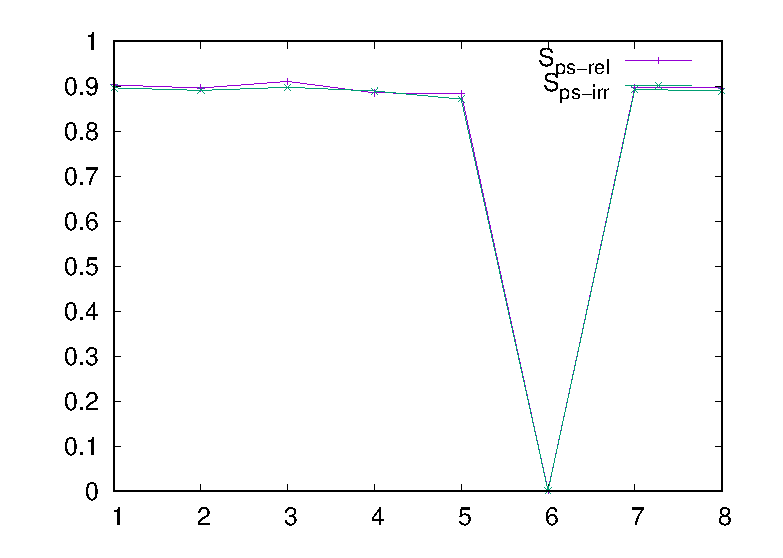
\includegraphics[scale=0.8]{313-1_scores.eps}}
    \caption{Оценки релевантности для модели без ограничений на поисковыую выдачу}\label{fig:wv-scores-1}
\end{figure}

\begin{figure}
    \centerline{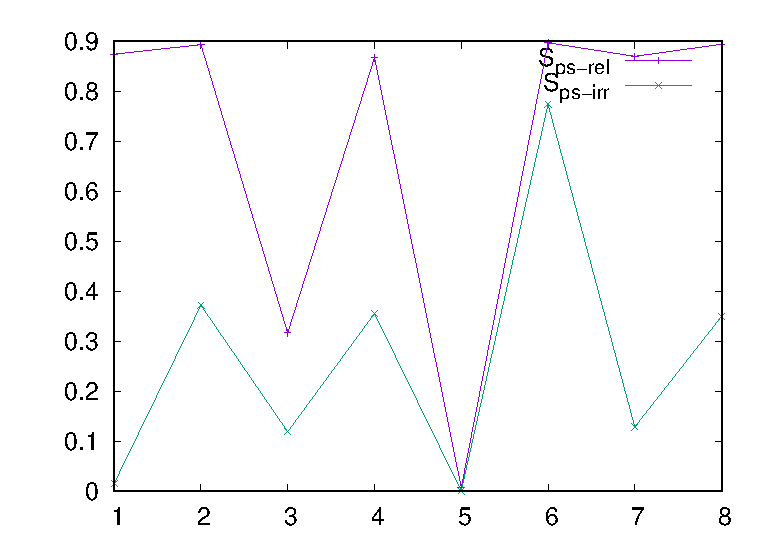
\includegraphics[scale=0.8]{313-2_scores.eps}}
    \caption{Оценки релевантности для модели с примененными ограничениями}\label{fig:wv-scores-2}
\end{figure}